This chapter shows some examples of \LaTeX{} writing.

\section{Equations}
There are several commands to write equations such as \textbackslash{}equation, \textbackslash{}eqnarray, and \textbackslash{}align.
This section shows examples of \textbackslash{}align as
\begin{align}
y = Ax+b.
\label{eq:exampleSingle}
\end{align}
You can refer any equation by using \textbackslash{}ref command as 式~\ref{eq:exampleSingle}.
This thesis template defines a useful command \textbackslash{}eref \eref{eq:exampleSingle}.

\par
\textbackslash{}align can shows multiple equations as
\begin{align}
y &= Ax+b ,
\label{eq:exampleMultiple1} \\
x &= K[R|t]X.
\label{eq:exampleMultiple2}
\end{align}
It is possible to assign a label to each equation as \eref{eq:exampleMultiple1} and \eref{eq:exampleMultiple2}.

\par
Matrix can be written by \textbackslash{}matrix commands.
When you need bracket (or parenthesis), you can use \textbackslash{}bmatrix (or \textbackslash{}pmatrix) as
\eref{eq:exampleMatrix}
\begin{align}
  P = 
	\begin{bmatrix}
		p_{11} & p_{12} & p_{13} & p_{14} \\
		p_{21} & p_{22} & p_{23} & p_{24} \\
		p_{31} & p_{32} & p_{33} & p_{34} 
	\end{bmatrix}.
\label{eq:exampleMatrix}
\end{align}

\section{Figures}
Here's an example how to put a figure.
Each figure should have a caption, which explains the contents of the figure, below the figure.
The size of a figure is adjustable by specifying its size.
In this example, the size is set as the width of the figure equals 60\% of column width. 
Same as equations, you can refer any figure by using \textbackslash{}ref command as 図~\ref{fig:example}.
This thesis template defines a useful command \textbackslash{}fref as \fref{fig:example}.
\begin{figure}[tb]
	\centering
		
\includegraphics[width=0.6\hsize]{example-figure}
		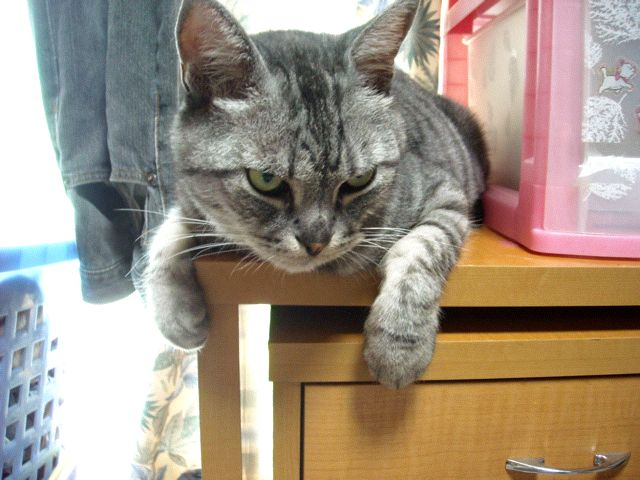
\includegraphics[width=0.6\hsize]{cat}
	\caption{Example of figure}
	\label{fig:example}
\end{figure}

\section{Tables}
Here's an example how to put a table.
Again, you can refer any table by using \textbackslash{}ref command as Table~\ref{tab:example}.
This thesis template defines a useful command \textbackslash{}tref as \tref{tab:example}.
More complicated table is shown in \tref{tab:example2}.
\begin{table}[tb]
	\centering
		\caption{Example of table}
		\begin{tabular}{r|c|c}
			\hline
			name & id & size \\
			\hline \hline
			John Doe & 1 & 100 \\
			Jane Doe & 3 & 150 \\
			\hline
		\end{tabular}
	\label{tab:example}
\end{table}
\begin{table}[tb]
\begin{center}
\caption{Exmple of complicated table}
\begin{tabular}{l|cc|cc||cc|cc||cc|cc}
\hline\hline
& \multicolumn{4}{c||}{pretest} & \multicolumn{4}{c||}{posttest} & \multicolumn{4}{c}{Gain} \\
\cline{2-13}
& \multicolumn{2}{c|}{Score} & \multicolumn{2}{c||}{Time} & \multicolumn{2}{c|}{Score} & \multicolumn{2}{c||}{Time} & \multicolumn{2}{c|}{Score} & \multicolumn{2}{c}{Time} \\
\hline
Group     & A     & P     & A    & P  & A     & P     & A    & P  & A     & P     & A    & P \\
\hline
Mean      & 18.48 & 14.59 & 5.25 & 5.28 & 28.52 & 21.89 & 3.95 & 4.28 & 10.04 & 7.30 & 1.30 & 1.12 \\
Std. dev. & 10.93 & 11.52 & 1.44 & 1.23 &  5.63 &  9.92 & 1.17 & 1.16 &  8.85 & 7.85 & 1.12 & 1.15 \\
\hline
p & \multicolumn{2}{c|}{0.21} & \multicolumn{2}{c||}{0.89} & \multicolumn{2}{c|}{0.00} & \multicolumn{2}{c||}{0.32} & \multicolumn{2}{c|}{0.23} & \multicolumn{2}{c}{0.22} \\
\hline\hline
\end{tabular}
\label{tab:example2}
\end{center}
\end{table}

\section{Algorithms}
Here's an example how to put an algorithm.
Same as figure, you can refer any table by using \textbackslash{}ref command as Algorithm~\ref{alg:example}.
This thesis template defines a useful command \textbackslash{}aref as \alref{alg:example}.
\alref{alg:example2} shows another type of algorithm which contains normal text.
See \href{http://en.wikibooks.org/wiki/LaTeX/Algorithms}{here} for more detail about algorithm, algorithmicx, and algorithm2e packages.
\begin{algorithm}
	 \caption{Example of algorithm copied from \href{http://www.math-linux.com/latex-26/faq/latex-faq/How-to-write-algorithm-and}{here}}
	\label{alg:example}
	\begin{algorithmic}
		\REQUIRE $n \geq 0 \vee x \neq 0$
		\ENSURE $y = x^n$
		\STATE $y \leftarrow 1$
		\IF{$n < 0$}
			\STATE $X \leftarrow 1 / x$
			\STATE $N \leftarrow -n$
		\ELSE
			\STATE $X \leftarrow x$
			\STATE $N \leftarrow n$
		\ENDIF
		\WHILE{$N \neq 0$}
			\IF{$N$ is even}
				\STATE $X \leftarrow X \times X$
				\STATE $N \leftarrow N / 2$
			\ELSE[$N$ is odd]
				\STATE $y \leftarrow y \times X$
				\STATE $N \leftarrow N - 1$
			\ENDIF
		\ENDWHILE
	\end{algorithmic}
\end{algorithm}

\begin{algorithm}
	\caption{Example of algorithm with text copied from \href{ftp://ftp.u-aizu.ac.jp/pub/tex/CTAN/macros/latex/contrib/algorithms/algorithms.pdf}{here}}
	\label{alg:example2}
	\begin{algorithmic}
		\IF{some condition is true}
		\STATE do some processing
		\ELSIF{some other condition is true}
		\STATE do some different processing
		\ELSIF{some even more bizarre condition is met}
		\STATE do something else
		\ELSE
		\STATE do
		\ENDIF
	\end{algorithmic}
\end{algorithm}


\section{Reference}
Citation can be done by \textbackslash{}cite command as \cite{Adamowicz92} and \cite{AlloucheSh92,BartonFi72a,CaludeP83}.
For citation, it is highly recommended to use BibTeX.
For more flexible bibliography, you can use \href{http://www.ctan.org/pkg/natbib}{natbib}.


